\documentclass[12pt,a4paper,onecolumn]{article}
\usepackage[utf8]{inputenc}
\usepackage[T1]{fontenc}
\usepackage[french]{babel}

% ------------------------- Color table ----------------------------------------
\usepackage{multirow}
\usepackage[table]{xcolor}
\definecolor{maroon}{cmyk}{0,0.87,0.68,0.32}
% ------------------------------------------------------------------------------

\usepackage{amscd}
\usepackage{amsthm}
\usepackage{physics}
\usepackage[left=2.2cm,right=2.2cm,top=2cm,bottom=2cm]{geometry}
\usepackage{textcomp,gensymb} %pour le °C, et textcomp pour éviter les warning
\usepackage{graphicx} %pour les images
\usepackage{caption}
\usepackage{subcaption}
\usepackage[colorlinks=true,
	breaklinks=true,
	citecolor=blue,
	linkcolor=blue,
	urlcolor=blue]{hyperref} % pour insérer des liens
\usepackage{epstopdf} %converting to PDF
\usepackage[export]{adjustbox} %for large figures

\usepackage{array}
\usepackage{dsfont}% indicatrice : \mathds{1}


% -------------------------- Mathematics ---------------------------------------
\graphicspath{{images/}{../images/}} % For the images path
% ------------------------------------------------------------------------------

% -------------------------- Mathematics ---------------------------------------
\usepackage{mathrsfs, amsmath, amsfonts, amssymb}
\usepackage{bm}
\usepackage{mathtools}
\usepackage[Symbol]{upgreek} % For pi \uppi different from /pi
\newcommand{\R}{\mathbb{R}} % For Real space

% ------------------------------------------------------------------------------


% -------------------------- Code format ---------------------------------------
\usepackage[numbered,framed]{matlab-prettifier}
\lstset{
	style              = Matlab-editor,
	basicstyle         = \mlttfamily,
	escapechar         = '',
	mlshowsectionrules = true,
}
% ------------------------------------------------------------------------------

% ------------------------- Blbiographie --------------------------------------
% \usepackage[backend=biber, style=science]{biblatex}
% \addbibresource{biblio.bib}
% ------------------------------------------------------------------------------


\setcounter{tocdepth}{4} %Count paragraph
\setcounter{secnumdepth}{4} %Count paragraph
\usepackage{float}

\usepackage{graphicx} % for graphicspath
% \graphicspath{{../images/}}

\usepackage{array,tabularx}
\newcolumntype{L}[1]{>{\raggedright\let\newline\\\arraybackslash\hspace{0pt}}m{#1}}
\newcolumntype{C}[1]{>{\centering\let\newline\\\arraybackslash\hspace{0pt}}m{#1}}
\newcolumntype{R}[1]{>{\raggedleft\let\newline\\\arraybackslash\hspace{0pt}}m{#1}}

% to start counting section to 6


% ------------------------ General informations --------------------------------
\title{MVA - 3D Computer Vision - Disparity using graph cuts}
\author{Vincent Matthys}
\graphicspath{{images/}{../images/}{gcdispar/}} % For the images path
% ------------------------------------------------------------------------------


\begin{document}

\begin{tabularx}{0.9\textwidth}{@{} l X r @{} }
	{\textsc{Master MVA}}       &  & \textsc{Vincent Matthys} \\
	\textsc{3D Computer vision} &  & {ENS Paris Saclay}       \\
\end{tabularx}
\vspace{1.5cm}
\begin{center}

	\rule[11pt]{5cm}{0.5pt}

	\textbf{\LARGE \textsc{Disparity map estimation using graph cuts}}
	\vspace{0.5cm}

	Vincent Matthys

	vincent.matthys@ens-paris-saclay.fr

	\rule{5cm}{0.5pt}

	\vspace{1.5cm}
\end{center}

\tableofcontents

\clearpage

Ce rapporte accompagne le programme \textit{stereoGC} d'estimation de carte de disparité à partir de deux vues d'une même scène. Afin d'executer ce programme, il faut dans un premier temps lancer les commandes suivantes

\begin{lstlisting}[numbers = none]
cmake CMakeLists.txt
make
\end{lstlisting}

Qui produit un executable dans le répertoire courant \textit{stereoGC}. On exécute le programme sur deux images \textit{im1} et \textit{im2} de la façon suivante :

\begin{lstlisting}[numbers = none]
./stereoGC im1 im2
\end{lstlisting}

Deux utilisations modèles sont utilisables en définissant dans le préambule le \textit{define} correspondants :
\begin{itemize}
	\item THIERRY : charge les deux images du visage de Thierry ainsi que les paramètres raisonnables associés ; en particulier on se limite à une recherche de disparité \(d \in [10, 55]\).
	\item TOYS : charge les deux images de la scène des jouets ainsi que les paramètre raisonnables associés  ; en particulier on se limite à une recherche de disparité \(d \in [-30, -7]\).
\end{itemize}

Le rapport qui suit regroupe différentes observations quand à son utilisation sur différentes images et avec différents paramètres.

\section{Présentation de cas fonctionnels}

\subsection{Résultats pour Thierry}

En figure~\ref{fig_thierry_initial} sont présentées les deux vues de Thierry à partir desquelles la carte de disparité à été calculée.

\begin{figure}[H]
	\centering
	\begin{subfigure}[b]{0.45\textwidth}
		\centering
		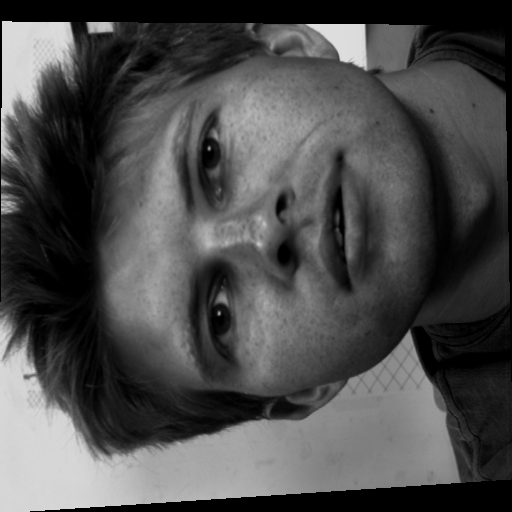
\includegraphics[width = \textwidth, angle = -90]{face00R}
		\caption{Première vue}
		\label{fig_thierry_1}
	\end{subfigure}
	\centering
	\begin{subfigure}[b]{0.45\textwidth}
		\centering
		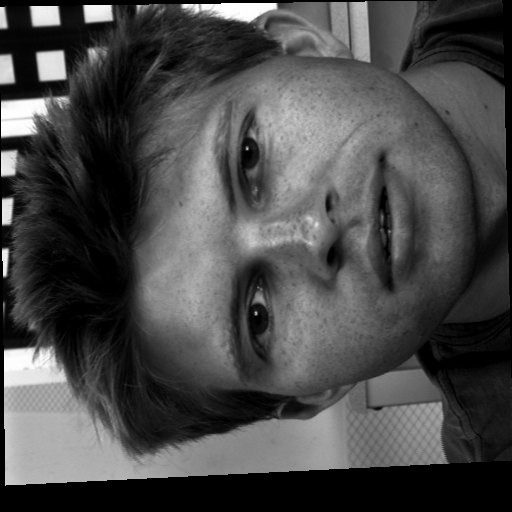
\includegraphics[width = \textwidth, angle = -90]{face01R}
		\caption{Deuxième vue}
		\label{fig_thierry_2}
	\end{subfigure}
	\caption{Les deux vues de Thierry à partir desquelles la carte de dispartié \ref{fig_thierry_3D} est calculée}
	\label{fig_thierry_initial}
\end{figure}

La carte de dispartié obtenue est présentée en figure~\ref{fig_thierry_3D}. On constate que le résultat est réaliste, suffisamment lisse mais rendant compte des informations pertinentes.

\begin{figure}[H]
	\centering
	\includegraphics[width = 0.9\textwidth]{thierry_3D_usecase}
	\caption{Carte de dispartié obtenue avec \(\sigma = 3\), \(w_{cc} = 20\), \(n = 7\)}
	\label{fig_thierry_3D}
\end{figure}

\subsection{Influence de la valeur du poids entre pixel non corrélés}

En figure~\ref{fig_thierry_wcc} est présenté l'influence du poids \(w_{cc}\) entre pixels non corrélés sur la carte de disparité. Pour ces expériences, on fixe \(n = 3\) et \(\sigma = 3\). Théoriquement, ce poids influence le niveau de discrétisation de l'énergie du graphe. En pratique, comme visible en figure~\ref{fig_thierry_disp_wcc_1000}, si ce poids est trop élevé, alors les variations de disparités entraînent une grande variation d'énergie, que le lissage ne suffit pas à compenser.

\begin{figure}[H]
	\centering
	\begin{subfigure}[b]{0.3\textwidth}
		\centering
		\includegraphics[height = 0.2\textheight, angle = -90]{thierry_disp_blur_3_z_2}
		\caption{\(w_{cc} = 20\)}
		\label{fig_thierry_disp_wcc_20}
	\end{subfigure}
	\centering
	\begin{subfigure}[b]{0.3\textwidth}
		\centering
		\includegraphics[height = 0.2\textheight, angle = -90]{thierry_disp_wcc_100}
		\caption{\(w_{cc} = 100\)}
		\label{fig_thierry_disp_wcc_100}
	\end{subfigure}
	\centering
	\begin{subfigure}[b]{0.3\textwidth}
		\centering
		\includegraphics[height = 0.2\textheight, angle = -90]{thierry_disp_wcc_1000}
		\caption{\(w_{cc} = 1000\)}
		\label{fig_thierry_disp_wcc_1000}
	\end{subfigure}
	\centering
	\begin{subfigure}[b]{0.3\textwidth}
		\centering
		\includegraphics[height = 0.2\textheight]{thierry_3D_blur_3_z_2}
		\caption{\(w_{cc} = 20\)}
		\label{fig_thierry_3D_wcc_20}
	\end{subfigure}
	\centering
	\begin{subfigure}[b]{0.3\textwidth}
		\centering
		\includegraphics[height = 0.2\textheight]{thierry_3D_wcc_100}
		\caption{\(w_{cc} = 100\)}
		\label{fig_thierry_3D_wcc_100}
	\end{subfigure}
	\centering
	\begin{subfigure}[b]{0.3\textwidth}
		\centering
		\includegraphics[height = 0.2\textheight]{thierry_3D_wcc_1000}
		\caption{\(w_{cc} = 1000\)}
		\label{fig_thierry_3D_wcc_1000}
	\end{subfigure}
	\caption{Carte de disparité obtenue pour différentes valeurs de poids entre pixels non corrélés \(w_{cc}\)}
	\label{fig_thierry_wcc}
\end{figure}


\subsection{Influence de la valeur de lissage}

En figure~\ref{fig_thierry} est présenté le résultat obtenu pour différentes valeurs de lissage. Pour ces expériences, on fixe \(n = 3\) et \(w_{cc} = 20\). On constate que les valeurs 3, 5 et 8 donnent des résultats similaires pour cette reconstruction. En revanche, comme attendu, des valeurs trop faibles de \(\sigma\) donne des discontinuités omniprésentes. A l'inverse, une trop grande valeur de lissage fait perdre de l'information.

\begin{figure}[H]
	\centering
	\begin{subfigure}[b]{0.3\textwidth}
		\centering
		\includegraphics[height = 0.2\textheight, angle = -90]{thierry_disp_blur_1_z_2}
		\caption{\(\sigma = 1\)}
		\label{fig_thierry_disp_1}
	\end{subfigure}
	\hfill
	\begin{subfigure}[b]{0.3\textwidth}
		\centering
		\includegraphics[height = 0.2\textheight, angle = -90]{thierry_disp_blur_2_z_2}
		\caption{\(\sigma = 2\)}
		\label{fig_thierry_disp_2}
	\end{subfigure}
	\hfill
	\begin{subfigure}[b]{0.3\textwidth}
		\centering
		\includegraphics[height = 0.2\textheight, angle = -90]{thierry_disp_blur_3_z_2}
		\caption{\(\sigma = 3\)}
		\label{fig_thierry_disp_3}
	\end{subfigure}
	\hfill
	\begin{subfigure}[b]{0.3\textwidth}
		\centering
		\includegraphics[height = 0.2\textheight]{thierry_3D_blur_1_z_2}
		\caption{\(\sigma = 1\)}
		\label{fig_thierry_3D_1}
	\end{subfigure}
	\hfill
	\begin{subfigure}[b]{0.3\textwidth}
		\centering
		\includegraphics[height = 0.2\textheight]{thierry_3D_blur_2_z_2}
		\caption{\(\sigma = 2\)}
		\label{fig_thierry_3D_1}
	\end{subfigure}
	\hfill
	\begin{subfigure}[b]{0.3\textwidth}
		\centering
		\includegraphics[height = 0.2\textheight]{thierry_3D_blur_3_z_2}
		\caption{\(\sigma = 3\)}
		\label{fig_thierry_3D_1}
	\end{subfigure}
	\hfill
	\begin{subfigure}[b]{0.3\textwidth}
		\centering
		\includegraphics[height = 0.2\textheight, angle = -90]{thierry_disp_blur_5_z_2}
		\caption{\(\sigma = 5\)}
		\label{fig_thierry_disp_5}
	\end{subfigure}
	\hfill
	\begin{subfigure}[b]{0.3\textwidth}
		\centering
		\includegraphics[height = 0.2\textheight, angle = -90]{thierry_disp_blur_8_z_2}
		\caption{\(\sigma = 8\)}
		\label{fig_thierry_disp_8}
	\end{subfigure}
	\hfill
	\begin{subfigure}[b]{0.3\textwidth}
		\centering
		\includegraphics[height = 0.2\textheight, angle = -90]{thierry_disp_blur_15_z_2}
		\caption{\(\sigma = 15\)}
		\label{fig_thierry_disp_15}
	\end{subfigure}
	\hfill
	\begin{subfigure}[b]{0.3\textwidth}
		\centering
		\includegraphics[height = 0.2\textheight]{thierry_3D_blur_5_z_2}
		\caption{\(\sigma = 5\)}
		\label{fig_thierry_3D_5}
	\end{subfigure}
	\hfill
	\begin{subfigure}[b]{0.3\textwidth}
		\centering
		\includegraphics[height = 0.2\textheight]{thierry_3D_blur_8_z_2}
		\caption{\(\sigma = 8\)}
		\label{fig_thierry_3D_8}
	\end{subfigure}
	\hfill
	\begin{subfigure}[b]{0.3\textwidth}
		\centering
		\includegraphics[height = 0.2\textheight]{thierry_3D_blur_15_z_2}
		\caption{\(\sigma = 15\)}
		\label{fig_thierry_3D_15}
	\end{subfigure}
	\caption{Carte de disparité obtenue pour différentes valeurs de lissage \(\sigma\)}
	\label{fig_thierry}
\end{figure}


\section{Comparaison avec l'expansion de graines}


En figure~\ref{fig_toys_initial} sont présentées l'image gauche et l'image droite de la scène de jouets à partir desquelles la carte de disparité à été calculée.

\begin{figure}[H]
	\centering
	\begin{subfigure}[b]{0.45\textwidth}
		\centering
		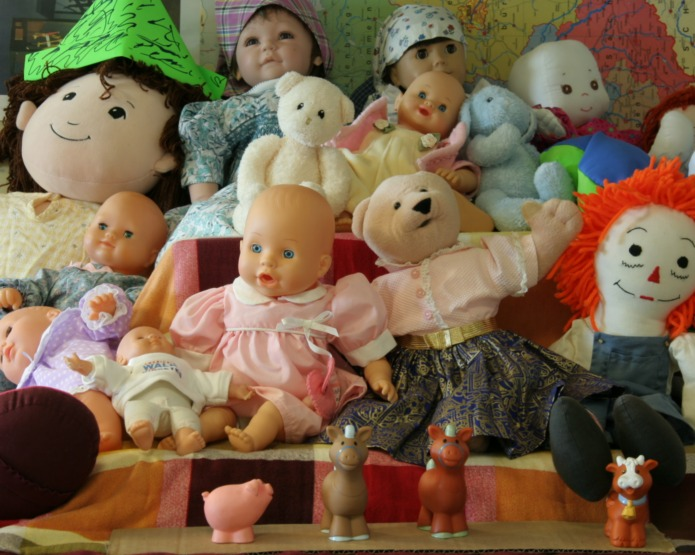
\includegraphics[width = \textwidth]{toys01}
		\caption{Vue de gauche}
		\label{fig_toys_1}
	\end{subfigure}
	\centering
	\begin{subfigure}[b]{0.45\textwidth}
		\centering
		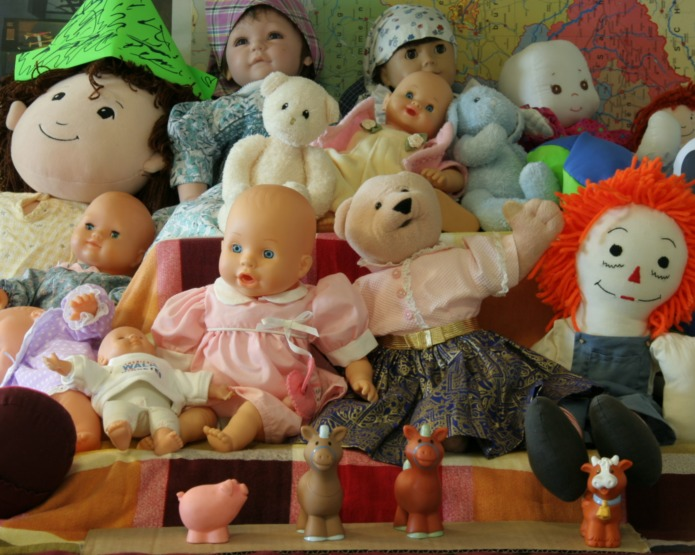
\includegraphics[width = \textwidth]{toys02}
		\caption{Vue de droite}
		\label{fig_toys_2}
	\end{subfigure}
	\caption{Les deux vues de la scène de jouets à partir desquelles la carte de dispartié \ref{fig_toys_3D} est calculée}
	\label{fig_toys_initial}
\end{figure}

La carte de dispartié obtenue est présentée en figure~\ref{fig_toys_3D}, et on peut la comparer à celle obtenue par expansion de graines visible en figure~\ref{fig_seeds_3D} : les niveaux de disparités recherchés sont, dans les deux cas, dans l'intervalle \([-30, -7]\). Il faut faire abstraction du fait que les niveaux de disparité pour la méthode par expansion n'est pas lissée. On constate néanmoins de gros défaut sur la méthode par expansion, notamment quand on visualise la carte de dispartié de profil, avec un nombre non négligeable de niveaux de disparité aberrants, qu'on ne retrouve pas par la méthode par graph cuts.

Le temps d'exécution de la méthode par graph cuts est de \(54~s\) avec un facteur de zoom 2, quand la méthode par expansion de graine prend \(69~s\). En définitif, la méthode par graph cuts, plus rapide à condition de prendre un facteur de zoon raisonnable, doit être correctement paramétrisé pour obtenir des résultats plus corrects que la méthode par expansion de graines.

\begin{figure}[H]
	\centering
	\includegraphics[height = 0.4\textheight]{toys_disp}
	\includegraphics[height = 0.4\textheight]{toys_3D}
	\caption{Carte de dispartié obtenue avec \(\sigma = 3\), \(w_{cc} = 20\), \(n = 7\) et un facteur de zoom 2}
	\label{fig_toys_3D}
\end{figure}


\begin{figure}[H]
	\centering
	\includegraphics[height = 0.4\textheight]{seeds_3D_1}
	\includegraphics[height = 0.4\textheight]{seeds_3D}
	\caption{Carte de dispartié obtenue par expansion de graines pour la même taille de fenêtre \(n = 7\)}
	\label{fig_seeds_3D}
\end{figure}


\end{document}
